% This is a sample document using the University of Minnesota, Morris, Computer Science
% Senior Seminar modification of the ACM sig-alternate style. Much of this content is taken
% directly from the ACM sample document illustrating the use of the sig-alternate class. Certain
% parts that we never use have been removed to simplify the example, and a few additional
% components have been added.

% See https://github.com/UMM-CSci/Senior_seminar_templates for more info and to make
% suggestions and corrections.

\documentclass{sig-alternate}
\usepackage{color}
\usepackage[colorinlistoftodos]{todonotes}

%%%%% Uncomment the following line and comment out the previous one
%%%%% to remove all comments
%%%%% NOTE: comments still occupy a line even if invisible;
%%%%% Don't write them as a separate paragraph
%\newcommand{\mycomment}[1]{}

\begin{document}

% --- Author Metadata here ---
%%% REMEMBER TO CHANGE THE SEMESTER AND YEAR AS NEEDED
\conferenceinfo{UMM CSci Senior Seminar Conference, April 2019}{Morris, MN}

\title{An Analysis of IoT System Applications on Global Public Health Issues}

\numberofauthors{1}

\author{
% The command \alignauthor (no curly braces needed) should
% precede each author name, affiliation/snail-mail address and
% e-mail address. Additionally, tag each line of
% affiliation/address with \affaddr, and tag the
% e-mail address with \email.
\alignauthor
David Chong\\
	\affaddr{Division of Science and Mathematics}\\
	\affaddr{University of Minnesota, Morris}\\
	\affaddr{Morris, Minnesota, USA 56267}\\
	\email{chong050@morris.umn.edu}
}

\maketitle
\begin{abstract}
In this paper I detail information needed in order to understand an Internet of Things (IoT) system. I then examine researchers efforts in designing systems to detect potentially problematic mosquito populations. I then examine security concerns from the perspective of designing a resilient smart home.
\end{abstract}

\keywords{Internet of Things}

\section{Introduction}
\label{sec:introduction}

The Internet of Things is a frequent topic of interest in the Computer Science disipline; but it is often talked about in vague terms. I will be detailing what is an IoT system, what goals IoT systems have, how those goals can be met, and some concerns that come up when discussing IoT systems.
% Not really happy with this part

I will be analyzing a few real world use cases of IoT systems. I will discuss differences between the systems and why certain requirements are needed in some while not in others.

\section{Background}
\label{sec:background}

%Here I need to talk about hardware acceleration, algorithms and big O, autovectorize and parallel computing and threading
%May briefly talk about various IoT devices like Intel Edison, Particle Photon, and Raspberry Pi

\subsection{Algorithms}
\label{sec:algorithms}

% Here I need to cover big O in order to analyze psudocode later on
This is quite a verbose topic so I will only be dipping our toes on this subject in order to later explain efficiency of a program in a meaningful way. When looking at a program we can think of each command as a step. Each step can be measured using big O. Big O is used to measure the run time of a function in terms of n -- the number of passes required to complete a computation. This measurement can be linear, quadratic, logarithmic, etc. This important to consider when needing to optimize the efficiency of a program. 

\subsection{Systems}
\label{sec:systems}

% Here I need to cover auto-vectorize, parallel computing and threading
Parallel computing is a valuable asset when designing a system. Use of parallel computing allows the system to perform multiple processes at the same time. Internet of Things devices may need to process vast amounts of data. Usage of parallel computing, and more specifically automatic vectorization lends way to more efficient systems. Automatic vectorization can be thought of as performing multiple steps at once. Consider a for loop that iterates one by one and computes a simple addition problem then sets that value equal to a unique variable. Automatic vectorization would allow for a defined number of those iterations to be performed similtaniously. One can imagine four  steps happening at once.

\subsection{Hardware Acceleration}
\label{sec:hardwareAcceleration}

% Here I need to cover hardware acceleration
When designing a system one must consider the hardware they will be using to implement said system. If possible, hardware acceleration can be used in order to have a system work more efficiently. It does this by using hardware like a computer's graphics card in order to process information rather than leaving all the work to the CPU. This is important later on as a system I will cover has the goal of being both efficient computationally and power consumption wise.

\subsection{Cryptography}
\label{sec:cryptography}

% Here I might talk about symmetric key cryptography as it is mentioned in both the secure data provenance and IoT security challenges articles

\subsection{Devices and IoT structure}
\label{sec:devices}

% Here I need to cover the different devices so that people understand later on when they are mentioned

Some of the devices used in the implementation of IoT systems include: Raspberry Pi 3, Intel Edison, cellular phones, etc. Any internet connected device can be considered an IoT device so keep in mind this list is far from exhaustive. The specifications of each device can vary greatly in terms of CPU clock speeds, system memory, flash memory, voltage requirements, and more. All these factors and more must be considered when designing an IoT system.

IoT is made up of three layers: preception, network and application. The preception layer includes the physical devices which collect information from various other devices in order to then send that information to the network layer. The network layer is the connection between the preception and application layers. The application layer takes the information from the network layer and processes it in a way that is likely valuable to an end user.

These devices are able to communicate using various methods such as RFID, NFC, Bluetooth, WIFI, and more. Each method of communication has its own various specifications such as frequency and range. Some of these methods are available on devices while others are not so that must be considered when designing an IoT system.

% Talk about cloud computing and providers
% Talk about Iaas, PaaS, SaaS

\section{Example A: Mosquito Detection - an IoT system}
\label{sec:mosquito}

In our first example, Ravi et al. were able to design an IoT system that was able to detect mosquito populations with an 80\% accuracy. There were able to achieve this using tiny board computers like Intel Edison and Raspbery Pi 3. Their main goal was to create a system that would be able to detect mosquito populations more efficiently than current methods. More granular goals included: keeping cost per device low, maintain high efficency through various optimizations -- this in turn creates another goal of maintaining low power usage in order to not need to service remote devices.

The researchers needed to first decide which devices would best suit their application. The main deciding factor here was how long the battery would last as the devices are ment to be used in remote locations such as mines, swamps, etc. 

%Here I am going to add possibly figure 2 (Need to explain FFT, kNN, and bayesian classifier at least briefly) and definitly figure 3 from the mosquito article.

\begin{figure}
\centering
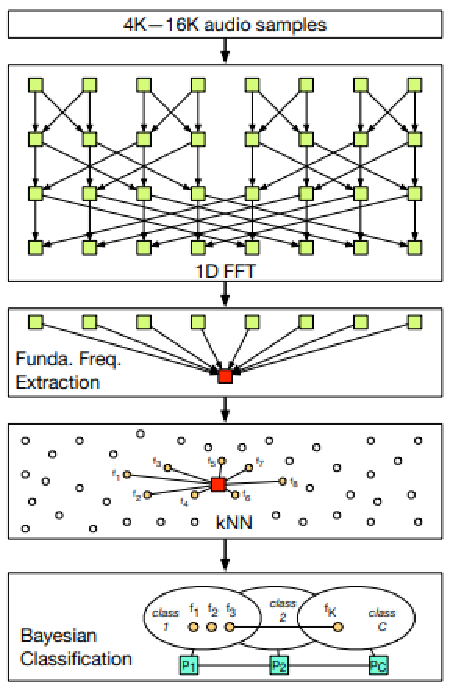
\psfig{file=imagetopdf1.pdf,width =3in}
\caption{A sample graph just spanning one column.}
\label{fig:singleColumnFigure1}
\end{figure}

The previous figure give us a view of how data is processed in order to get meaningful data from the mosquito measurements. Each sample must be processed through the three steps in order to accuratly classify and code the data. The researchers found this embedded computation method to be 80 times more energy efficient than using radio communication of the raw data. This method provides around two months of usage versus the radio methods mere 20 hours on a 2000 mAh AA battery on an Intel Edison. It is worth mentioning here -- the system sends data once per day and remains in a low power standby when not computing or sending data.

%Here I want to analyze the big O for the pseudocode

\begin{figure*}
\centering
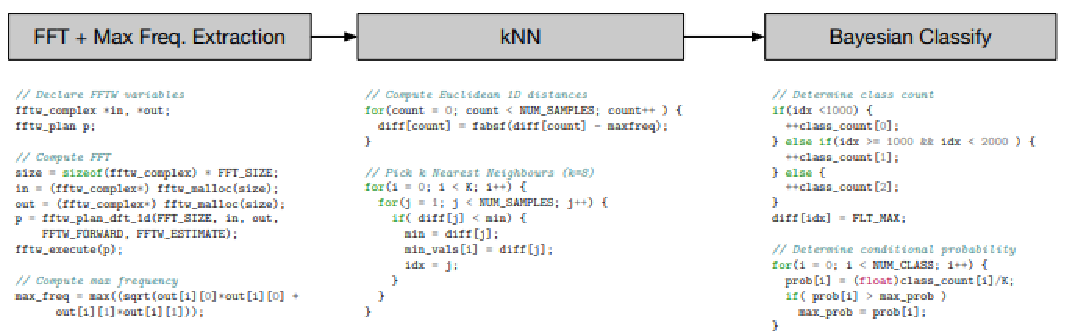
\psfig{file=imagetopdf2.pdf,width =5.3in}
\caption{A sample graph that needs to span two columns of text.}
\label{fig:twoColumnFigure1}
\end{figure*}

The researchers were able to identify that 80-90\% of the runtime was taken up by the FFT component -- see above figure. They were able to determine that usage of hardware accelerators were able to speed up the computation of this step by a factor of two.

The researchers also found that a trade off between precision and power usage would be valuable to the system. Originally their implementation used 32 bit floating-point hardware. This ment that computation on this data would be slower and require more storage -- both of these factors reduce the overall energy efficiency of the device. This prompted the researchers to instead choose to use 16 bit fixed point as their primary data type. They determined that this trade off would be worth the loss in precision in this specific case.

The researchers found they were able to add flags to their code in order to further optimize compiliation. An example of this would be use of the -msse2 flag. This allows the code to auto-vectorize and run parts in parallel. %this needs to be better explained
Other optimizations such as loop unrolling, reassociation and other arithmetic transformations due to use of compiler flags allow for further trade offs to be made granting higher speed of computation and less energy usage while losing precision. The researches found this acceptable with the caveat that overall classification accuracy remained unaffected.

These optimizations are both made on the hardware and the software.

%Here I want to import figure 6 from the mosquito article -- un-opt has no flags, opt1 has single threading, opt2 has multithreading - need to talk about hardsware optimizations

\begin{figure}
\centering
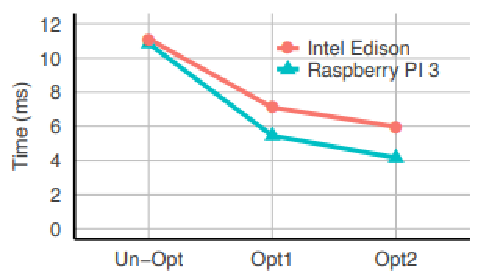
\psfig{file=imagetopdf3.pdf,width =3in}
\caption{A sample graph just spanning one column.}
\label{fig:singleColumnFigure2}
\end{figure}

%Need to explain FFT, kNN, and bayesian classifier at least briefly or above - needed in order to talk about software optimizations
%Will summarize the figures here rather than show

\begin{figure}
\centering
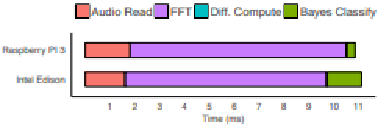
\psfig{file=imagetopdf4.pdf,width =3in}
\caption{A sample graph just spanning one column.}
\label{fig:singleColumnFigure2}
\end{figure}

In the end; the researchers were able to design a system which they say could be used in tandem with existing insect classification efforts in order to provide a more rich set of data to help identify the problematic mosquito populations quickly.

\section{Example B: Resillient Smart Home - IoT security}
\label{sec:home}

% Talk about issues that can arise in IoT systems and their causes
% Internet is unavailable
% Note this is very rough and needs to be cleaned up

It is important to consider how one would go about designing an IoT system that is resilient. It is not out of the realm of possibility that a system could lose connection to the internet due to any number of causes.

Causes for internet outage: technical problems, natural causes, targeted attacks. All of these lend way to possible negative effects such as lack of service, possibly providing an attack window on the system, or allowing unauthorized access. It is also important to note that a system may need manual intervention in order to run properly after an outage occurs. All of these reasons point to a need for resilient IoT systems, especially in cases where safety is a main concern. One of the articles I read in preperation for this paper details several functions that may be used in IoT systems in order to provide a more resilient system. These functions include: the ability to detect cloud failure, providing a notification, or performing a service transfer. This list is far from exhaustive but provides an idea of possible solutions available to help aid the resilience issue.

When designing an IoT system it is important to identify services provided which one would consider essential. We must design around these essential services in order to provide acceptable service in case of external failure such as internet disconnection.

The earlier that security is considered when designing a IoT system the better. Security issues can quickly snowball out of control especially with certain IoT systems as they could be designed to be easily scaleable. If the issue is unfound and deployed to a wide audience it is difficult address after the fact as the inital problem becomes obsured over time. It is also possible that issues may lie within the hardware or software creating another layer of obsurity in terms of identifying root security flaws.

While tamper and fault resistance are not mandatory in terms of functionality of an IoT system they are still important to consider as each layer of defense makes attacks on the system more difficult to carry out. Network attacks that take advantage of computational phenomena such as instance cache attacks, timing attacks, and faults induced by the Row hammer approach are all possible and must be considered when designing an IoT system.

As IoT grows as a fairly new idea we must consider the vast amount of data, some of which can be sensitive, making IoT systems lucrative targets to cybercriminals. The systems running these devices can be limited making security requirements difficult to manage.

Main challenges: authentication, data integrity, data provenance, privacy, and access control. These devices are sometimes deployed remotely so physical security of the device must also be noted. This means that security against both physical and network attacks must be designed for.

% Talk about physical unclonable functions (PUFs) and how they ensure data provenance

\section{Test}
\label{sec:test}
This is a test to see how much more I need to add to meet the four page requirements for this cookie deadline. This is a test to see how much more I need to add to meet the four page requirements for this cookie deadline. This is a test to see how much more I need to add to meet the four page requirements for this cookie deadline. This is a test to see how much more I need to add to meet the four page requirements for this cookie deadline. This is a test to see how much more I need to add to meet the four page requirements for this cookie deadline. This is a test to see how much more I need to add to meet the four page requirements for this cookie deadline. This is a test to see how much more I need to add to meet the four page requirements for this cookie deadline. This is a test to see how much more I need to add to meet the four page requirements for this cookie deadline. This is a test to see how much more I need to add to meet the four page requirements for this cookie deadline. This is a test to see how much more I need to add to meet the four page requirements for this cookie deadline. 

\section*{Acknowledgments}
\label{sec:acknowledgments}

I would like to thank professors Lamberty and Machkasova for there countinuous help and feedback throughout this course. I would  like to thank the other professors in the CSCI faculty as well. I would also like to thank my friends and family who have helped me through the process of my Senior Seminar.

% The following two commands are all you need in the
% initial runs of your .tex file to
% produce the bibliography for the citations in your paper.
\bibliographystyle{abbrv}
% sample_paper.bib is the name of the BibTex file containing the
% bibliography entries. Note that you *don't* include the .bib ending here.
\bibliography{sample_paper}  
% You must have a proper ".bib" file
%  and remember to run:
% latex bibtex latex latex
% to resolve all references

\end{document}

\section{The {\secit Body} of The Paper}
\label{sec:body}

Typically, the body of a paper is organized
into a hierarchical structure, with numbered or unnumbered
headings for sections, subsections, sub-subsections, and even
smaller sections.  The command \texttt{\textbackslash section} that
precedes this paragraph is part of such a
hierarchy.\footnote{This is the second footnote.  It
starts a series of three footnotes that add nothing
informational, but just give an idea of how footnotes work
and look. It is a wordy one, just so you see
how a longish one plays out.} \LaTeX\ handles the numbering
and placement of these headings for you, when you use
the appropriate heading commands around the titles
of the headings.  If you want a sub-subsection or
smaller part to be unnumbered in your output, simply append an
asterisk to the command name.  Examples of both
numbered and unnumbered headings will appear throughout the
balance of this sample document.

Because the entire article is contained in
the \textbf{document} environment, you can indicate the
start of a new paragraph with a blank line in your
input file; that is why this sentence forms a separate paragraph.

\subsection{Type Changes and {\subsecit Special} Characters}
\label{sec:typeChangesSpecialChars}

We have already seen several typeface changes in this sample.  You
can indicate italicized words or phrases in your text with
the command \texttt{\textbackslash textit}; emboldening with the
command \texttt{\textbackslash textbf}
and typewriter-style (for instance, for computer code) with
\texttt{\textbackslash texttt}.
As a rule you'd prefer \texttt{\textbackslash emph} (which stands for \emph{emphasize})
over something like \texttt{\textbackslash textit} since that gives the typesetting system
more flexibility in how it can emphasize that text.

You do not
have to indicate typestyle changes when such changes are
part of the \textit{structural} elements of your
article; for instance, the heading of this subsection will
be in a sans serif\footnote{A third footnote, here.
Let's make this a rather short one to
see how it looks.} typeface, but that is handled by the
document class file. Take care with the use
of\footnote{A fourth, and last, footnote.}
the curly braces in typeface changes; they mark
the beginning and end of
the text that is to be in the different typeface.

You can use whatever symbols, accented characters, or
non-English characters you need anywhere in your document;
you can find a complete list of what is
available in the \textit{\LaTeX\
User's Guide}~\cite{Lamport:LaTeX}.

\subsection{Math Equations}
\label{sec:mathEquations}

You may want to display math equations in three distinct styles:
inline, numbered or non-numbered display.  Each of
the three are discussed in the next sections.

\subsubsection{Inline (In-text) Equations}
\label{sec:inlineEquations}

A formula that appears in the running text is called an
inline or in-text formula.  It is produced by the
\textbf{math} environment, which can be
invoked with the usual \texttt{\textbackslash begin\ldots\textbackslash end}
construction or with the short form \texttt{\$\ldots \$}. You
can use any of the symbols and structures,
from $\alpha$ to $\omega$, available in
\LaTeX~\cite{Lamport:LaTeX}; this section will simply show a
few examples of in-text equations in context. Notice how
this equation: \begin{math}\lim_{n\rightarrow \infty}x=0\end{math},
set here in in-line math style, looks slightly different when
set in display style.  (See next section).

\subsubsection{Display Equations}
\label{sec:displayEquations}

A numbered display equation -- one set off by vertical space
from the text and centered horizontally -- is produced
by the \textbf{equation} environment. An unnumbered display
equation is produced by the \textbf{displaymath} environment.

Again, in either environment, you can use any of the symbols
and structures available in \LaTeX; this section will just
give a couple of examples of display equations in context.
First, consider the equation, shown as an inline equation above:

\begin{equation*}
\lim_{n\rightarrow \infty}x=0
\end{equation*}

Notice how it is formatted somewhat differently in
the \textbf{displaymath}
environment.  Now, we'll enter an unnumbered equation:

\begin{displaymath}
	\sum_{i=0}^{\infty} x + 1
\end{displaymath}

and follow it with a numbered equation (Equation~\ref{eq:summation}):

\begin{equation}
	\sum_{i=0}^{\infty}x_i=\int_{0}^{\pi+2} f
\label{eq:summation}
\end{equation}

just to demonstrate \LaTeX's able handling of numbering.
Note that if you use numbered equations, you can give them \texttt{label}s
and \texttt{\textbackslash ref} them, e.g., Equation~\ref{eq:summation}.

\subsection{Multi-line formulas}
\label{sec:multiLineFormulas}

The \texttt{align} and \texttt{align*} environments let you align sequences of
equations so, for examples, a sequences of equal signs line up nicely. 

% The & creates a "virtual tab stop" and corresponding &'s on each line
% will be aligned when the layout is done.
\begin{align*}
n_1 &= \sum_{i = 1}^k a_i \\
n_{x-y} &= \prod_{i = 1}^k b_i
\end{align*}

\begin{align*}
 f(x) &= (x+a)(x+b) \\
 &= x^2 + (a+b)x + ab
\end{align*}

\subsection{Figures}
\label{sec:figures}

Like tables, figures cannot be split across pages; the
best placement for them
is typically the top or the bottom of the page nearest
their initial cite.  To ensure this proper ``floating'' placement
of figures, use the environment
\textbf{figure} to enclose the figure and its caption.

This sample document contains examples of
a \textbf{.pdf} file to be displayable with \LaTeX, such as
Figure~\ref{fig:singleColumnFigure}.  More
details on each of these is found in the \textit{Author's Guide}.

\begin{figure}
\centering
\psfig{file=sample_graph.pdf,width =3in}
\caption{A sample graph just spanning one column.}
\label{fig:singleColumnFigure}
\end{figure}


As was the case with tables, you may want a figure
that spans two columns, like Figure~\ref{fig:twoColumnFigure}.  
To do this, and still to
ensure proper ``floating'' placement of tables, use the environment
\texttt{figure*} to enclose the figure and its caption.
And don't forget to end the environment with
\texttt{figure*}, not \texttt{figure}!

\begin{figure*}
\centering
\psfig{file=sample_graph.pdf,width =5.3in}
\caption{A sample graph that needs to span two columns of text.}
\label{fig:twoColumnFigure}
\end{figure*}

It's easiest and you tend to get the best quality if your figure uses vector graphics
in PDF format. You can include other formats such as PNG, but they will usually
not look nearly as professional, especially when printed on high resolution printers.
\emph{Be very wary of screen captures from other papers. They tend to look pixelated
and amateurish even at high resolutions.}

\subsection{Tables}
\label{sec:tables}

Because tables cannot be split across pages, the best
placement for them is typically the top of the page
nearest their initial cite.  To
ensure this proper ``floating'' placement of tables, use the
environment \textbf{table} to enclose the table's contents and
the table caption.  The contents of the table itself must go
in the \textbf{tabular} environment, to
be aligned properly in rows and columns, with the desired
horizontal and vertical rules.  Again, detailed instructions
on \textbf{tabular} material
is found in the \textit{\LaTeX\ User's Guide}.

Immediately following this sentence is the point at which
Table~\ref{tab:frequencyOfSpecialChars} is included in the input file; 
compare the placement of the table here with the table in the
PDF output running \LaTeX\ on this document.

\begin{table}[t]
\centering
\caption{Frequency of Special Characters}
\label{tab:frequencyOfSpecialChars}
\begin{tabular}{c|c|l}
Non-English or Math & Frequency & Comments\\ \hline
\O & 1 in 1,000 & For Swedish names\\
$\pi$ & 1 in 5 & Common in math\\
\$ & 4 in 5 & Used in business\\
$\Psi^2_1$ & 1 in 40,000 & Unexplained usage\\
\end{tabular}
\end{table}

To set a wider table, which takes up the whole width of
the page's live area, use the environment
\textbf{table*} to enclose the table's contents and
the table caption, as demonstrated in Table~\ref{tab:typicalCommands} below.  
As with a single-column table, this wide
table will ``float" to a location deemed more desirable.
Immediately following this sentence is the point at which
Table~\ref{tab:typicalCommands} is included in the input file; again, it is
instructive to compare the placement of the
table here with the table in the printed dvi
output of this document.


\begin{table*}[t]
\centering
\caption{Some Typical Commands}
\label{tab:typicalCommands}
\begin{tabular}{ccl}
Command & A Number & Comments \\ \hline
\texttt{\textbackslash alignauthor}     & 100 & Author alignment\\
\texttt{\textbackslash numberofauthors} & 200 & Author enumeration\\
\texttt{\textbackslash table}           & 300 & For tables\\
\texttt{\textbackslash table*}          & 400 & For wider tables\\ 
\end{tabular}
\end{table*}
% end the environment with {table*}, NOTE not {table}!


\subsection{Citations}
\label{sec:citations}

Citations to articles~\cite{Aaronson:2005,Garey:1979,Brun:2008} listed
in the Bibliography section of your
article will occur throughout the text of your article.
You should use BibTeX to automatically produce this bibliography;
you simply need to insert one of several citation commands with
a key of the item cited in the proper location in
the \texttt{.tex} file~\cite{OM:2008}.
The key is a short reference you invent to uniquely
identify each work; in this sample document, the key is
the first author's surname and a
word from the title.  This identifying key is included
with each item in the \texttt{.bib} file for your article.

It is recommended that you precede \texttt{\textbackslash cite} (and 
\texttt{\textbackslash ref}) commands with a tilde
character instead of a space, e.g., \texttt{some text\textasciitilde\textbackslash cite}. The tilde gives you a non-breaking space which ensures that your citation won't get
stranded by itself on the beginning of a line.

The details of the construction of the \texttt{.bib} file
are beyond the scope of this sample document, but more
information can be found in the \textit{Author's Guide},
and exhaustive details in the \textit{\LaTeX\ User's
Guide}.

This article shows only the plainest form
of the citation command, using \texttt{\textbackslash cite},
which is all that is needed for our senior seminar.
You shouldn't use any other forms here.

\subsection{Theorem-like Constructs}
\label{sec:theoremLikeConstructs}

Other common constructs that may occur in your article are
the forms for logical constructs like theorems, axioms,
corollaries and proofs.  There are
two forms, one produced by the
command \texttt{\textbackslash newtheorem} and the
other by the command \texttt{\textbackslash newdef}; perhaps
the clearest and easiest way to distinguish them is
to compare the two in the output of this sample document:

Theorem~\ref{thm:integration} below uses the \textbf{theorem} environment, created by
the \texttt{\textbackslash newtheorem} command:

% You would usually put a \newtheorem command up at the top 
% of your LaTeX document after the \usepackage commands. It's
% just here in this example so it's with the text that describes it.
\newtheorem{theorem}{Theorem}

\begin{theorem}
Let $f$ be continuous on $[a,b]$.  If $G$ is
an antiderivative for $f$ on $[a,b]$, then
\begin{displaymath}\int^b_af(t)dt = G(b) - G(a).\end{displaymath}
\label{thm:integration}
\end{theorem}

The other uses the \textbf{definition} environment, created
by the \texttt{\textbackslash newdef} command:
\newdef{definition}{Definition}
\begin{definition}
If $z$ is irrational, then by $e^z$ we mean the
unique number which has
logarithm $z$: \begin{displaymath}{\log e^z = z}\end{displaymath}
\end{definition}

Two lists of constructs that use one of these
forms is given in the
\textit{Author's  Guidelines}.
 
There is one other similar construct environment, which is
already set up
for you; i.e. you must \textit{not} use
a \texttt{\textbackslash newdef} command to
create it: the \textbf{proof} environment.  Here
is a example of its use:
\begin{proof}
Suppose on the contrary there exists a real number $L$ such that
\begin{displaymath}
\lim_{x\rightarrow\infty} \frac{f(x)}{g(x)} = L.
\end{displaymath}
Then
\begin{align*}
l &= \lim_{x\rightarrow c} f(x) \\
  &= \lim_{x\rightarrow c}
\left[ g{x} \cdot \frac{f(x)}{g(x)} \right ] \\
  &= \lim_{x\rightarrow c} g(x) \cdot \lim_{x\rightarrow c}
\frac{f(x)}{g(x)}  \\
  &= 0\cdot L  \\
  &= 0,
\end{align*}
which contradicts our assumption that $l\neq 0$.
\end{proof}

Complete rules about using these environments and using the
two different creation commands are in the
\textit{Author's Guide}; please consult it for more
detailed instructions.  If you need to use another construct,
not listed therein, which you want to have the same
formatting as the Theorem
or the Definition~\cite{salas:calculus} shown above,
use the \texttt{\textbackslash newtheorem} or the
\texttt{\textbackslash newdef} command,
respectively, to create it.

\subsection*{A {\secit Caveat} for the \TeX\ Expert}
\label{sec:caveatForExperts}

Because you have just been given permission to
use the \texttt{\textbackslash newdef} command to create a
new form, you might think you can
use \TeX's \texttt{\textbackslash def} to create a
new command: \textit{Please refrain from doing this!}
Remember that your \LaTeX\ source code is primarily intended
to create camera-ready copy, but may be converted
to other forms -- e.g. HTML. If you inadvertently omit
some or all of the \texttt{\textbackslash def}s recompilation will
be, to say the least, problematic.

\section{Conclusions}
\label{sec:conclusions}

This paragraph will end the body of this sample document.
Remember that you might still have Acknowledgments or
Appendices; brief samples of these
follow.  There is still the Bibliography to deal with; and
we will make a disclaimer about that here: with the exception
of the reference to the \LaTeX\ book, the citations in
this paper are to articles which have nothing to
do with the present subject and are used as
examples only.